\chapter{Presenting Proposed LPs}
\label{chapter4}

The Chapter will provide an analysis and in-depth presentation of LPs from Section \ref{ssec:table_of_combinations}.
In general, each profile has its use-case already assigned in Table \ref{tab:use_cases}.
Here, we will focus on exposing the main features, issues, and use cases of the aforementioned LPs. 

Using the same pattern as in Table \ref{fig:map_fig}, we will first present per-building LPs with different time ranges.
We will start with simple LPs and then move to more advanced LPs with two-time dimensions.
Secondly, using the same pattern, we will present per-appliance profiles.
Finally, we will present per-building per-appliance LPs.
Data for profiles in this chapter was used from building 2 from the REFIT dataset discussed in Section \ref{ssec:data}.
 
\section{Time Ranges}
\label{sec:time_range}

Time ranges are an important part of the LP since each reveals a different usage pattern.
Throughout the thesis, we used four different time ranges: daily, weekly, monthly and yearly.

The daily profiles are the most commonly used LPs, as can be seen in Table \ref{tab:contributions}
Generally, they are the easiest to build since they do not need as much data as others do.
To build a decent profile one needs enough data. 
A sufficient amount of data is the amount that covers major events.
For a daily profile, a few weeks of data is enough, weekly LPs need a few months of data, monthly few months, and yearly few years.
And this is the main issue, there is rarely enough data to build such profiles.
Even then, usage patterns could change over a long period such as a decade.
Combining that with a smaller number of use cases for such profiles, reveals why such profiles were not looked into as much in Table \ref{tab:contributions}.

One more thing about time ranges that need to be mentioned are patterns that they present.
Daily profiles present daily usage and enable us to extract contextual events such as waking up, cooking, leisure time, etc.
The weekly pattern is also repetitive, and it enables us to see how appliance usage changes over the weekdays and weekends.
The monthly profile has none of the above. It is not repetitive since each day of the month can be a different day of the week, and the period is too short to capture seasonal patterns.
Alternatively, it could be presented as a week in a month, but there is no significant usage pattern to be revealed.
The yearly profile on the other hand presents the seasonal effects on usage such as increased daylight and temperature. 

\section{Per-Building LPs}
\label{sec:per_building}
The section will be focused on per-building profiles.
Per-building profiles refer to representations where whole building usage is presented as a single LP.
This kind of presentation is useful for observing general activation trends in a building.
Possible use cases for per-building LPs are grid management and energy saving.

When it comes to activation LPs there is one issue compared to power LPs.
To build per-building power LPs it is possible to use the main power meter, whereas, at activation LPs, sub-meter or disaggregated data is needed.
This can be solved using NILM algorithms, but they are not in a state of practical use yet.

The daily per-building LP is also known as the standard LP. 
According to Table \ref{tab:contributions} this is the most commonly used power profile.
Figures \ref{fig:SLPdaily2} and \ref{fig:SLPyearly2} present usage patterns on different time ranges. 
The two profiles, therefore present different contextual cases.

\begin{figure}[H]
	\begin{subfigure}{.5\textwidth}
		% \centering
		\caption{Daily}
		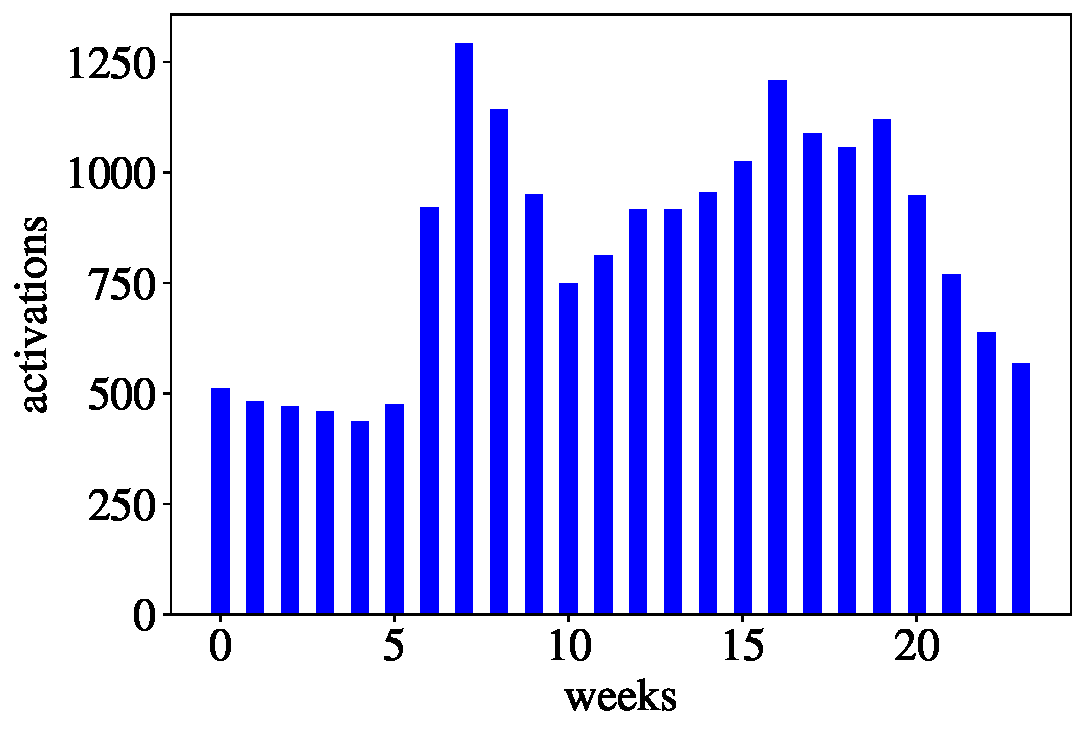
\includegraphics[width=1\linewidth]{../Figures/LPS/SLPdaily2.pdf}
		\label{fig:SLPdaily2}
	\end{subfigure}%
	~ 
	\begin{subfigure}{.5\textwidth}
		% \centering
		\caption{Yearly}
		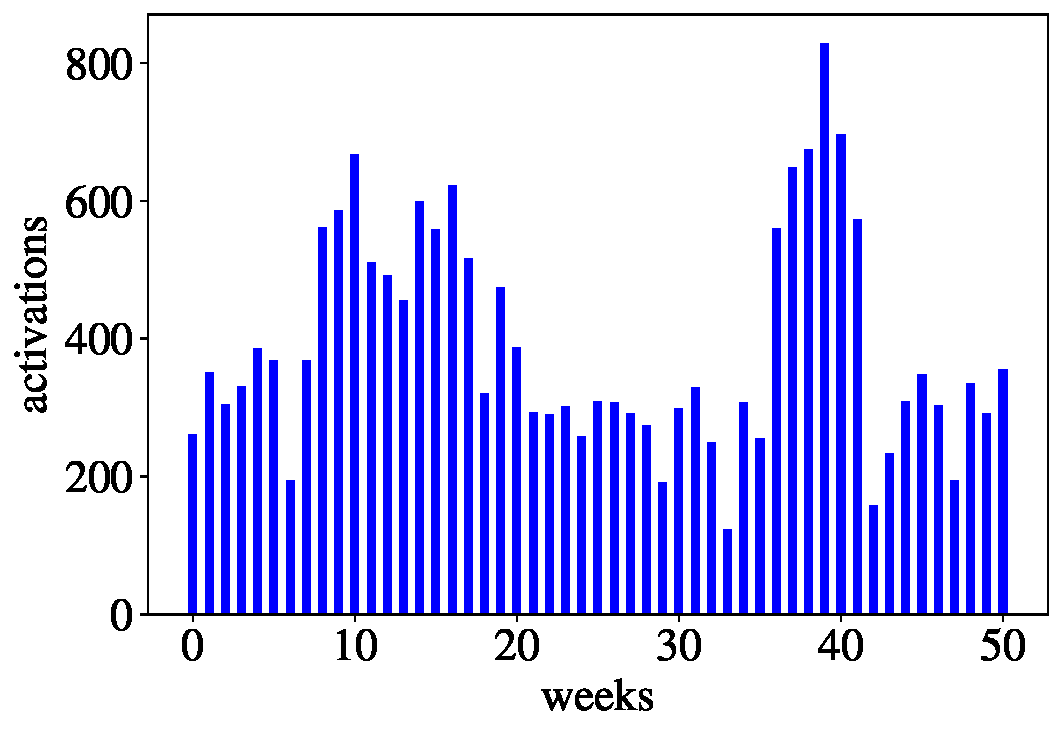
\includegraphics[width=1\linewidth]{../Figures/LPS/SLPyearly2.pdf}
		\label{fig:SLPyearly2}
	\end{subfigure}%
	\label{fig:SLP}
	\caption{Per-building LPs}
\end{figure}

The first Figure \ref{fig:SLPdaily2} shows how activations change throughout the day.
It is possible to see that there is some activity even throughout the night and early morning.
These can mostly be related to fridges or other appliances that are not directly activated by users.
At around 8 in the morning, it is possible to detect the first peak. 
These can be related to morning choirs. 
Then, at around noon, a dip occurs. 
The reason behind it is probably, that the dwellers are not home.
In the afternoon, the rate of activations slowly increases until it peaks at around 19 o'clock. 
This slow rise could be a contribution of each dweller arriving home at different parts of the day.

The second Figure \ref{fig:SLPyearly2} shows how activations change over the year.  
Again, it is possible to observe two peaks.
One in the spring and the other one in autumn. 
It is hard to correlate the activity with the seasonal effect since it seems like the activity is about the same in mid-winter as in mid-summer. 
The exact reason behind this pattern is unknown.

\subsection{Per-Building Two-Dimensional Time LPs}
\label{ssec:per_building_two_time_dim}
Alternatively, it is possible to combine Figures \ref{fig:SLPdaily2} and \ref{fig:SLPyearly2} and present activations as a heat map.
The result is a Figure \ref{fig:SLPHMyearly2} showing more complex activation patterns.

\begin{figure}[H]
	\centering
	\caption{Two-time-dimensional per-building LP}
	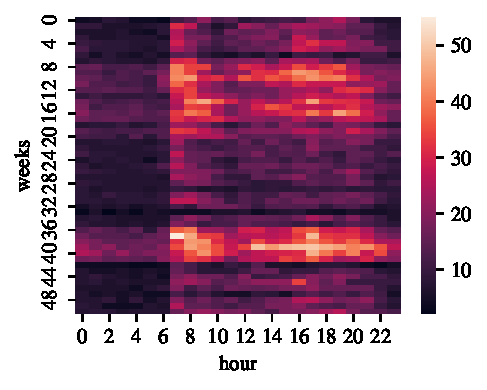
\includegraphics[width=0.7\textwidth]{../Figures/LPS/SLPHMyearly2.pdf}
	\label{fig:SLPHMyearly2}
\end{figure}


By combining the Figures and presenting them with a heat map, additional features are revealed.
For example, the black lines are the ones that probably present the vacation or other events where dwellers are away from home.

When analyzing Figure \ref{fig:SLPyearly2} it seems like dips in activity are for a similar reason, but Figure \ref{fig:SLPHMyearly2} shows these two dips from a different perspective.
The peak activity in Figure \ref{fig:SLPHMyearly2} shows a routine or a pattern similar to what was seen in \ref{fig:SLPdaily2}, one peak in the morning and one in the evening. 
The same pattern can be observed in winter dip, even though the pattern is less clear it is present.
The same cannot be said for the summer dip in the middle of the plot. 
Here, while the morning peak is visible, the evening one can barely be detected.

One more thing to mention is that the increased activity at the start of the fall increased activity throughout the night and day.
This could point to that some new appliance was installed, which increased the number of activations.

Previously, in Section \ref{sec:grid_managment}, it was mentioned that these kinds of profiles are the most applicable in grid management. 
One such example could be load shedding.
Using the LP above, electrical energy providers could find buildings with the least activity at that time of day.
Combining that with power data, it could disconnect the buildings with the least activity and most power consumption.

\section{Per-appliance}

Per-appliance LPs offer a look into the consumption of each appliance. 
In the case of activation LP, this is an elemental LP, since all other activation LPs are built on top of it. 
This also means that it is one of the most universal profiles since it can be used in use-cases defined in Section \ref{sec:use-cases}

\begin{figure}[H]
	\centering
	\caption{Daily per-appliance LP}
	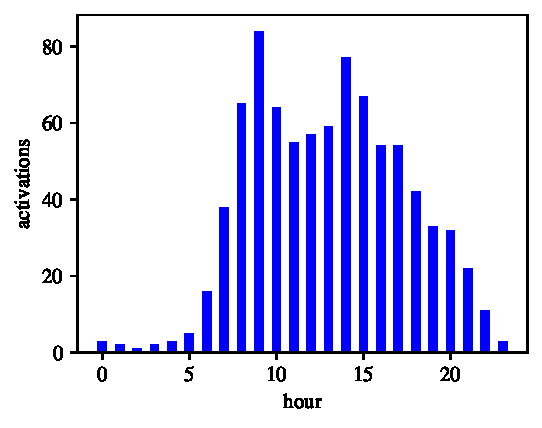
\includegraphics[]{../Figures/LPS/WM_daily.pdf}
	\label{fig:WM_daily}
\end{figure}

Looking at Figure \ref{fig:WM_daily}, we can detect a similar pattern as in per-building Figure \ref{fig:SLPdaily2}. 
While the peaks are closer together, the pattern remains.
One thing to notice here is, that the washing machine is used only throughout the day.
This means that this household does not use the cheaper nighttime tariffs.

Another parameter that was not explicitly mentioned before, is the resolution of LPs. 
Histograms can be presented using various resolutions or numbers of buckets.
An optimal number of buckets is a number that clearly presents the usage pattern. 
3-hour bucket size in Figure \ref{fig:4hours} does a good job at presenting the appliance usage at the main parts of the day.
This offers a better contextual presentation that is easier to process using algorithms.
As we can see in Figure \ref{fig:4hours}, by increasing the extent of buckets, the two peaks join together into one larger peak.
This coincides with the point of the presentation, where we want to present a more general pattern in key parts of the day.

\begin{figure}[H]
	\centering
	\caption{Daily per-appliance LP with larger buckets sizes}
	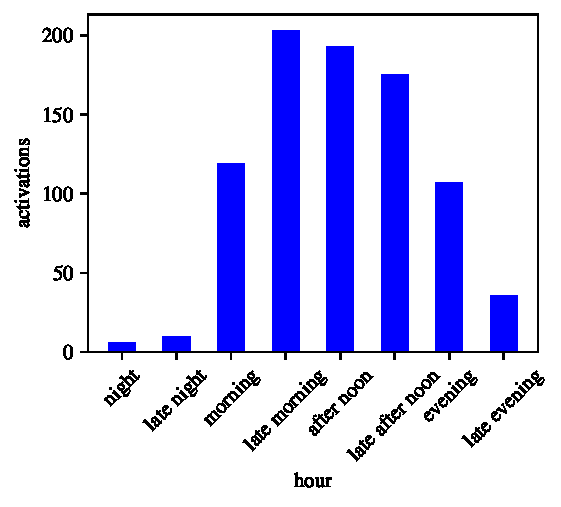
\includegraphics[]{../Figures/LPS/3_hours.pdf}
	\label{fig:4hours}
\end{figure}

While the low resolution is useful for contextual presentation,
high resolution is needed for time-sensitive applications such as elderly care,
where we have to detect an accident as soon as possible.
The hourly resolution would mean that in case of an accident, system would need at least an hour to detect it.
While this is sufficient for demonstrating the capabilities, real implementation would need to use lower-resolution data.

In the case where dwellers have different usage patterns during the weekends, two profiles would have to be developed.
It is possible to present them both at once such as in Figure \ref{fig:WM_ww_daily}. 
This is essentially a variation of the weekly LP that maintains high resolution.
Since there are more weekdays than weekend days, activations had to be normalized accordingly.

Figure \ref{fig:WM_ww_daily} again shows the same pattern as in Figure \ref{fig:WM_daily}.
What can we observe here is how these two patterns are the same but are shifted in time. 
On weekdays the first peak occurs at around 10 AM and the second at around 3 PM.
On weekends the first peak does not occur until 12 AM and the second at around 6 PM.
This shift in the pattern shows that while there is a change in behavior between weekends and weekdays it is not a
drastic one, at least in this case. 

\begin{figure}[H]
	\centering
	\caption{Normalized daily per-appliance with weekday and weekend LPs.}
	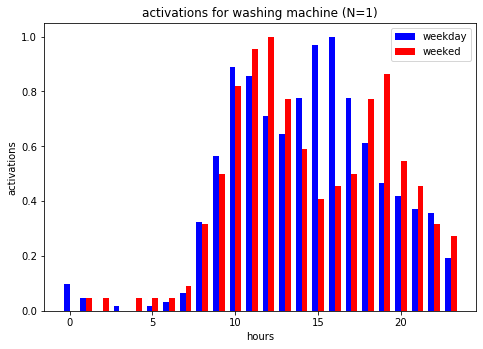
\includegraphics[width=0.7\textwidth]{../Figures/LPS/WM_ww_daily.png}
	\label{fig:WM_ww_daily}
\end{figure}

Another way to present weekly data is shown in Figure \ref{fig:WM_weekly}.
In this case, weekdays are numbered, where 0 stands for Monday and 6 for Sunday.
This resolution offers a look into how consumption pattern changes over the week. 
This is useful for applications such as grid management or energy saving.
In this particular case, it is possible to see that the user most commonly uses the washing machine on Mondays and Wednesdays.
Using a weekly weather report that would indicate high energy production on Wednesday, the electricity provider could offer a low cost for energy for that day. 
This kind of presentation could also be used to detect daily anomalies.

\begin{figure}[H]
	\centering
	\caption{Weekly per-appliance LP}
	\includegraphics[]{../Figures/LPS/WM_weekly.pdf}
	\label{fig:WM_weekly}
\end{figure}

In Section \ref{sec:time_range} we mentioned that the monthly presentation does not show any significant usage pattern, so it was not shown here. 
The yearly presentation again shows the more broad usage pattern, which can be seen in Figure \ref{fig:WM_yearly}.
This is useful for grid management and energy saving, where one could detect seasonal changes in the usage of an appliance. 

\begin{figure}[H]
	\centering
	\caption{Yearly per-appliance LP}
	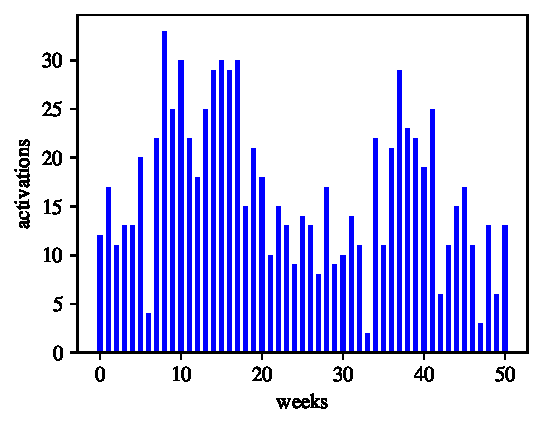
\includegraphics[]{../Figures/LPS/WM_yearly.pdf}
	\label{fig:WM_yearly}
\end{figure}

When comparing the pattern from Figure \ref{fig:WM_yearly} to pattern from Figure \ref{fig:SLPyearly2} 
it is possible to see the very same pattern. When making a quick comparison, they seem like the same image,
only when taking a closer look it is possible to see that differences do exists. 
We can make a similar conclusion here, as we did for Figure \ref{fig:SLPyearly2}.
It is hard to do any deeper analysis without the metadata.

\subsection{Two-Dimensional Time Per-Appliance LPs}

Using a combination of Figures \ref{fig:WM_daily} and \ref{fig:WM_weekly},
it is possible to generate Figure \ref{fig:wm_hm_weekly}.

\begin{figure}[H]
	\centering
	\caption{Two-dimensional time per-appliance LP}
	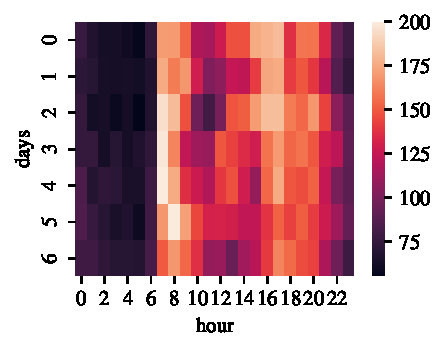
\includegraphics[]{../Figures/LPS/wm_hm_weekly.pdf}
	\label{fig:wm_hm_weekly}
\end{figure}
 
In this case, a similar use-case could be fitted as in the first example in Section \ref{ssec:per_building_two_time_dim}.
The first example used load shedding when the demand is too high.
On the contrary, it can also occur if the grid demand is too low.
There are two solutions to this issue.
The first one is to decrease production, which can be slow and expensive.
The second option is to load the grid, which can be done in many ways.
One of the ways is to turn on appliances using a direct load control system or notify users to turn on appliances that they have commonly used at that time in the past. 
Due to the increasing percentage of renewable energy sources, more and more energy peaks will be weather dependent.
By combining weekly wind forecasts, weekly cloud coverage, and user consumption profiles energy providers could notify users to turn on their appliances at peak usage times.

By analyzing Figure \ref{fig:wm_hm_weekly} it is possible to see that the user uses a washing machine,
on Wednesdays from 15 to 16 o'clock quite commonly. 
Should weather reports indicate high production peaks, the electrical provider could offer low-cost energy for that time of day for all users with similar usage patterns. 
This could all be automated for appliances such as home grid batteries, water heaters, EVs, or even fridges with a control system.
This would mean that the grid operator could regulate the demand instantly.
By using LPs it could prioritize appliances that would be used anyway, which would leave minimal impact on users' routines. 
While renewable energy is cheap to produce, it is expensive to store.
Increased adoption of such resources will require a large amount of energy to be stored and released, this process is at best 80 \% efficient.
If that energy is optimally distributed, less energy would be lost due to conversion.

\subsubsection{Other Two-Dimensional Presentations}

Figures \ref{fig:var_2d_lpss} show how some appliances have a constant usage pattern over a year, whereas again others change it. 
Examples below are randomly picked appliances from UK-DALE and REFIT. 

The Figure \ref{fig:HM_Ywh_comp} shows how computer usage changes over the year.
In the first quarter, the computer was used from 10:00 a.m. to 8:00 p.m.
In week 18 it is possible to observe that the computer is less and less used throughout the day. 
Starting week 40 it is again possible to see that the computer is getting more and more use in the morning hours. 
This is a good example of how can a usage pattern slowly change through the year. 
Since the pattern seems to bounce back, it could be seasonally correlated. 

The second example is Figure \ref{fig:HM_Ywh_tv}. It shows how TV usage changes over the year.
Compared to the computer, it is possible to see that the pattern looks a lot more persistent with slight changes.
Interestingly enough, when a close-up observation is made, it is possible to see that at the time when the computer was at its peak
the TV was at its low. And when the usage of computers decreased, the usage of TV increased. 
Due to the lack of metadata, it is hard to know the exact reason behind it. 

The good thing about this change is, that it takes a few weeks before it changes. 
This will be important later in Chapter \ref{chapter6} when we will be designing an elderly care system, that will be based on periodical user behavior.
This slow change gives the system time to adapt. 

One observation of quick behavior change can be made in weeks 8-11 and weeks 38-37, where we can see a black row on all three sub-Figures in Figure \ref{fig:var_2d_lpss}.
The instant decrease in activity is probably a vacation.

The last Figure is \ref{fig:HM_Ywh_wm} where the LP portrays the yearly use of the washing machine.
In this case, the seasonal pattern is much clearer. 
It seems like the appliance was used in the early morning hours of the winter and early spring.
This practice suddenly stops at week 13, until it appeared back in week 36.
  
\begin{figure}[H]
	\begin{subfigure}{.32\textwidth}
		\centering
		\caption{Computer}
		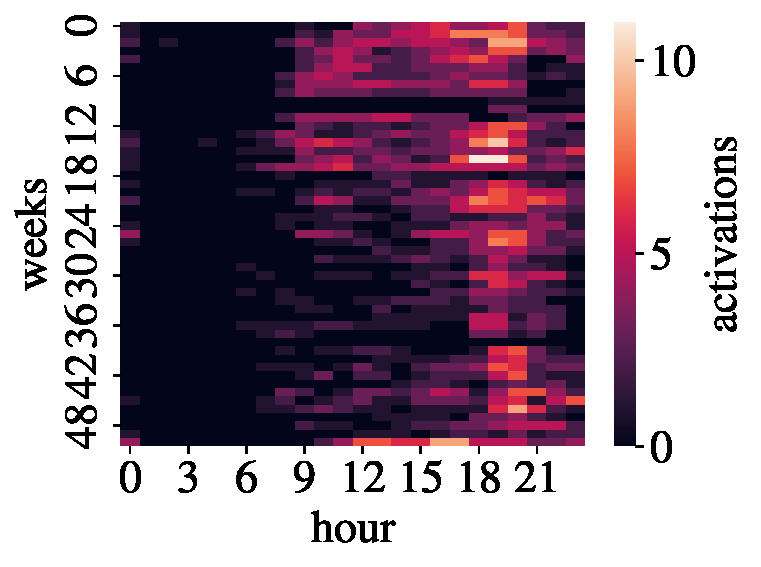
\includegraphics[width=1\textwidth]{../Figures/LPS/HM_Ywh_comp.pdf}
		\label{fig:HM_Ywh_comp}
	\end{subfigure}%
	\begin{subfigure}{.32\textwidth}
		\centering
		\caption{TV}
		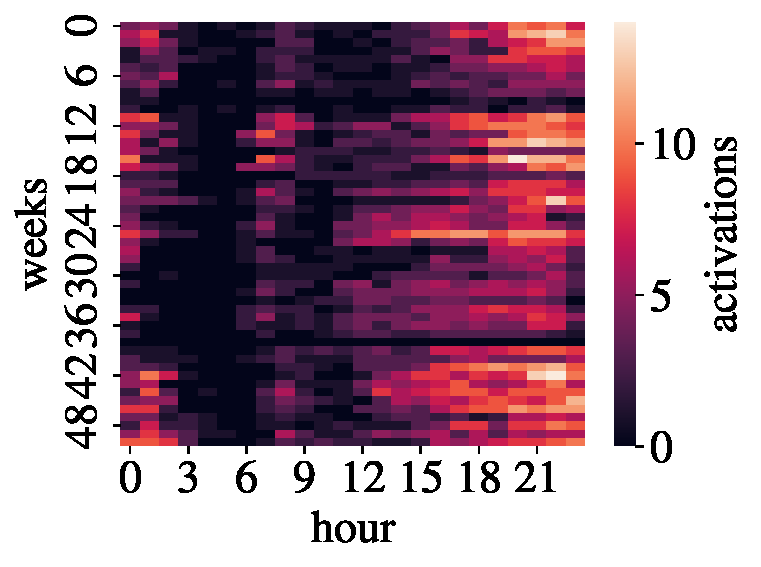
\includegraphics[width=1\textwidth]{../Figures/LPS/HM_Ywh_tv.pdf}
		\label{fig:HM_Ywh_tv}
	\end{subfigure}%
	\begin{subfigure}{.32\textwidth}
		\centering
		\caption{Washing machine}
		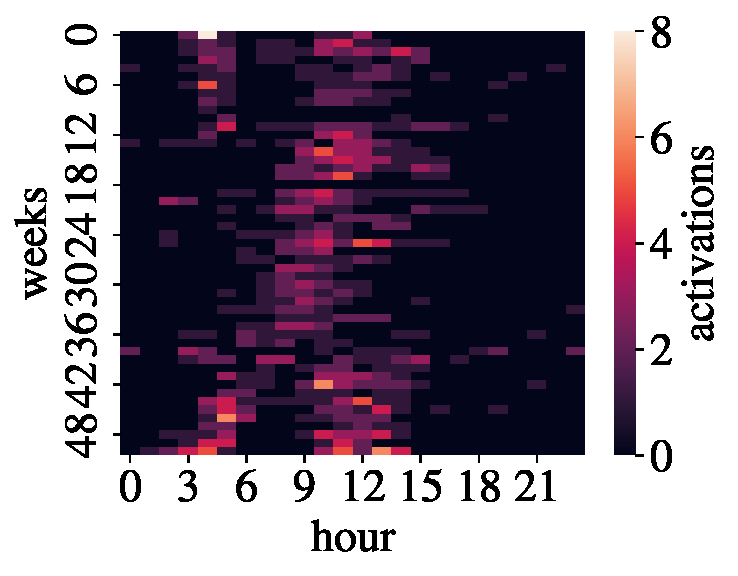
\includegraphics[width=1\textwidth]{../Figures/LPS/HM_Ywh_wm.pdf}
		\label{fig:HM_Ywh_wm}
	\end{subfigure}%
	
	\caption{Various yearly two-dimensional LPs for building 4 from REFIT.}
	\label{fig:var_2d_lpss}
\end{figure}

Another example worth mentioning is Figure \ref{fig:effect_of_season} from UK-DALE building 1, where data was collected from 2012-11-09 to 2017-04-26.
Roughly 5 years of data mean that it is possible to build a decent profile. 

\begin{figure}[H]
	\begin{subfigure}{.5\textwidth}
		\centering
		\caption{Solar thermal pumping station}
		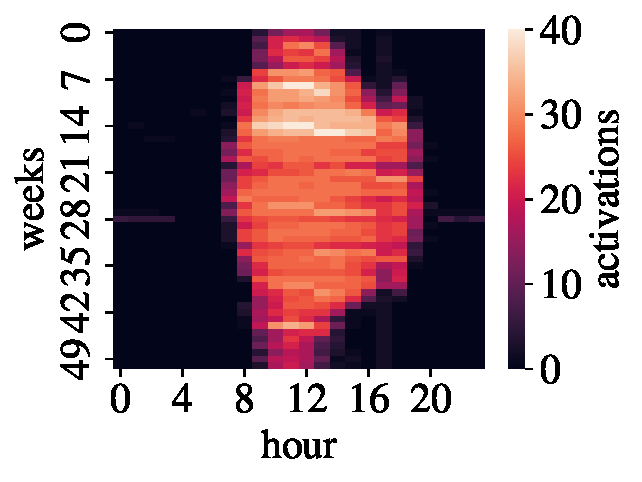
\includegraphics[width=0.9\textwidth]{../Figures/LPS/solar_thermal_pumping_station.pdf}
		\label{fig:solar_thermal_pumping_station}
	\end{subfigure}%
	\begin{subfigure}{.5\textwidth}
		\centering
		\caption{Light}
		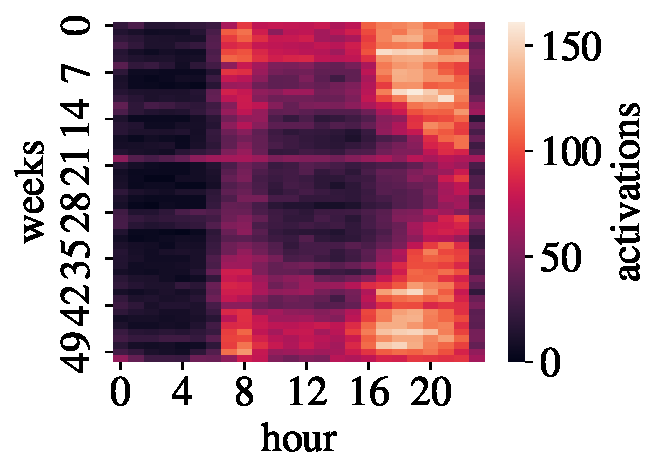
\includegraphics[width=0.9\textwidth]{../Figures/LPS/light.pdf}
		\label{fig:light}
	\end{subfigure}%
	\caption{Effect of seasonal changes on LPs}
	\label{fig:effect_of_season}

\end{figure} 

Appliance on Figure \ref{fig:solar_thermal_pumping_station} activates when water in solar collectors heats up to a certain threshold.
Since water heats up based on the strength of solar radiation, we can observe the change in solar radiation throughout the year for the UK. 

Appliance on Figure \ref{fig:light} on the other hand works quite the opposite.
We usually turn on the light when the solar radiation falls below a certain threshold, and turn it off when we sleep.
The Figure is one of the best examples, where we can observe the combined effect of user behavior, in this case sleeping, and the seasonal effect of changing solar radiation on users' behavior. 

Combining Figures \ref{fig:solar_thermal_pumping_station} and \ref{fig:light} enables us to differentiate between the two. 

\section{Per-Building Per-Appliance}

The last group of profiles is a combination of per-building and per-appliance LPs.
Observing the usage pattern of many appliances offers a better look into users' usage patterns.

In the case of elderly care, the goal is to observe a group of appliances.
Activation of a group of appliances would yield a contextual event.
If a stove and kettle are commonly used together each morning this use could translate to an event such as breakfast. 
To achieve this, one needs to observe all appliances at once such as shown in Figure \ref{fig:PHPA}.

Figure \ref{fig:PHPA} is also a good example of the elderly care system, that would detect an anomaly such as a fall, or a person unable to get up from the bed in the morning.
This profile shows that the first thing in the morning used are a kettle and toaster, and with a delay of one hour, microwave and TV. 
This enables us to construct time thresholds in which appliances should be used.
If none of these appliances are activated between set thresholds, morning would be considered anomalous.
Although less likely, issues could also occur during the use of appliances. 
In case an elder falls during cooking, toasting bread or opening the fridge the duty cycle would increase, which would also be considered an anomaly.
In case any of these anomalies are detected, the caregiver would be notified to check on the elder. 

\begin{figure}[H]
	\centering
	\caption{Daily per-appliance per-building building LP}
	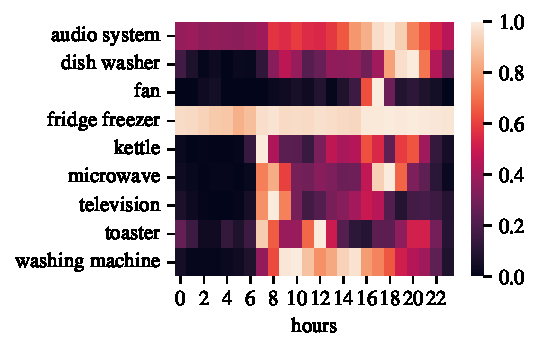
\includegraphics[]{../Figures/LPS/PHPA_profile_for_building.pdf}
	\label{fig:PHPA}
\end{figure}

The very same data can be presented in an alternative way, such as shown in Figure \ref{fig:stack}.
The usage pattern is the same as on \ref{fig:SLPdaily2}, except that it is possible to see
the contribution of each appliance. 

\begin{figure}[H]
	\centering
	\caption{Stacked daily per-appliance per-building building LP}
	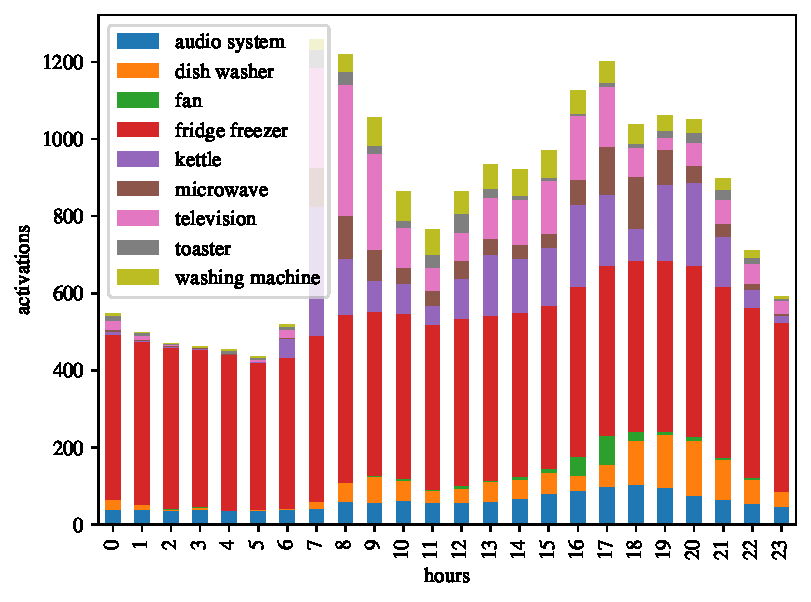
\includegraphics[width=.8\textwidth]{../Figures/LPS/stacked_LP.pdf}
	\label{fig:stack}
\end{figure}  
 
These LPs are useful when it comes to analyzing the usage pattern in one building.
To be able to process the LPs across many buildings a new profile, seen in Figure \ref{fig:BOA}, must be introduced.
The idea is derived from the bag-of-words method used in text processing, where a list of the most commonly used words is formed, and then used to process the text. 
Here, It is possible to use the activation data from all five datasets.
A list of appliances is sorted by the number of activations and then only the top 30 appliances are selected.
Using this list it is possible to present the usage of each building universally. This solves the issue of different appliances in different buildings.

\begin{figure}[H]
	\centering
	\caption{Universal presentation of per-building per-appliance LP}
	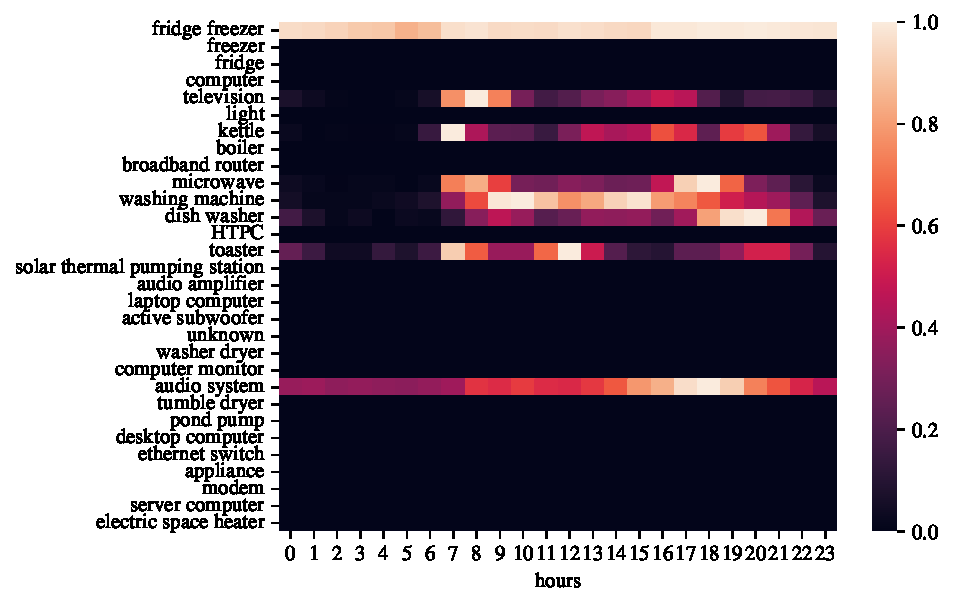
\includegraphics[width=1\textwidth]{../Figures/LPS/BOA.pdf}
	\label{fig:BOA}
\end{figure}

While analyzing Figure \ref{fig:BOA} we can see that the fridge freezer is most commonly activated.
Since there is no pattern, and it is activated randomly, the pattern is presented as a white line.
For the graph to be balanced, we have normalized the activations.
If we had not done this, we could observe only the fridge freezer, due to its activation dominance. 

Other, more dynamic appliances have a much clearer presentation of their activity. 
One other thing that we can notice is that there are a lot of empty LPs for certain appliances.
This is because we have no data for these appliances for this household.
Probably, this is one of the biggest weak points of this LP.

The Bag of appliances was not shown on the Table of profiles \ref{tab:our_rd},
since it is a special case of the per-building per-appliance profile shown in Figure \ref{fig:PHPA}.

\section{Summary}

This chapter showed how some activation profiles from Table \ref{tab:contributions} present real-world data, analyzed the presentations and further elaborated on their use-cases.

It was possible to see how each LP presents its unique user activation pattern. 
Figure \ref{fig:SLPdaily2} offered us a unique look into how users behave on daily basis and Figure \ref{fig:SLPyearly2} how this behavior changes over a year.
Next, with Figure \ref{fig:SLPHMyearly2}, we presented how combining these figures presents new features, that were otherwise hidden.
Further on it was shown how the very same presentations can be used on appliance data.
For example, Figure \ref{fig:effect_of_season} showed how this yearly change could be affected by the seasons.
Finally, we have shown how more detailed profiles \ref{fig:PHPA} could be used for practical applications such as elderly care. 